\documentclass[handout]{beamer}
\usepackage[utf8]{inputenc}
\usepackage{graphics}
\mode<presentation> {
\usetheme{unc}}
\setbeamertemplate{navigation symbols}{} % To remove the navigation symbols from the bottom of all slides uncomment this line

\usepackage{graphicx} % Allows including images
\usepackage{booktabs} % Allows the use of \toprule, \midrule and \bottomrule in tables


\usepackage{hyperref}
\hypersetup{linkcolor=blue,colorlinks=true}


% Remove symbols
\beamertemplatenavigationsymbolsempty


%\usetheme{default}

\usefonttheme{serif}

%----------------------------------------------------------------------------------------
%	TITLE PAGE
%----------------------------------------------------------------------------------------


\title[International Law and Human Rights]{\LARGE{International Law and Human Rights}}
\author[POLI 150]{Steven Saroka}
\institute{POLI 150}
\date{25 April 2024}


\begin{document}

\begin{frame}
\titlepage % Print the title page as the first slide
\end{frame}


%----------------------------------------------------------------------------------------
%	PRESENTATION SLIDES
%----------------------------------------------------------------------------------------

\begin{frame} 
	\frametitle{\LARGE{Announcements}}
	\begin{itemize}
		\item Final Exam to be available from 12 AM on April 30 through 11:59 PM on May 3. Cumulative, 15-20 multiple choice questions, open-note and open-book, 2 hour 30 minute time limit.
		\item Prompts 12 and 13 due on April 30.
	
	\end{itemize}
\end{frame}


\begin{frame} 
	\frametitle{\LARGE{Today's Class}}
	\begin{itemize}

			\item Intl. Law Definitions 

			\item Intl. Law Formation  

			\item Norms 

			\item Enforcement 

			\item What Are Human Rights?

			\item Human Rights Violations

			\item Why Do States Care?

			\item Rwandan Genocide and R2P

			\item The ICC
		
	\end{itemize}
\end{frame}

\begin{frame} 
	\frametitle{\LARGE{Key Terms}}
	\begin{itemize}
		\item International law
		\item Dimensions of international law
		\item Hard vs. soft law
		\item Norms
		\item Transnational Advocacy Networks (TANs)
		\item Boomerang model
		\item Human rights
		\item Negative and positive rights
		\item International Bill of Rights
		\item International Criminal Court
	\end{itemize}
\end{frame}

\begin{frame} 
	\frametitle{\LARGE{Central Questions of Intl Law}}
	\centering
	\Large{What is international law? How is it made? When and why do states follow it?}
\end{frame}


\begin{frame} 
	\frametitle{\LARGE{Geneva Conventions}}
	\begin{itemize}
		\item Signed in 1949, the \textbf{Geneva Conventions} are a set of international treaties describing what activities are ``legal" in war. \pause
		\item \textbf{This should be puzzling.}
	\end{itemize}
\end{frame}

\begin{frame} 
	\frametitle{\LARGE{Geneva Conventions}}
	\centering
	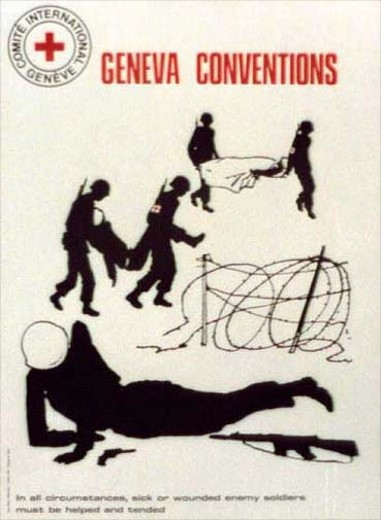
\includegraphics[width=\textwidth,height=\textheight,keepaspectratio]{GenevaCon.jpg}
\end{frame}

\begin{frame} 
	\frametitle{\LARGE{Geneva Conventions}}
	\begin{itemize}
		\item War is an exercise in attempting to kill the enemy. 
		\item Thus, war is fundamentally non-cooperative. \pause
		\item Yet, ``law" requires some amount of cooperation. How can there be “law” for such a violent and non-cooperative act?
		
	\end{itemize}
\end{frame}

\begin{frame} 
\frametitle{\LARGE{Definitions}}
\begin{itemize}
		\item \textbf{International law}: ``body of rules that binds states and other agents in world politics and is considered to have the status of law" (\textit{FLS} 465). \pause
		\item Effectively, international law is an \textbf{institution} that shapes how states perceive their interests.
		\item International law can enable cooperation between states through clear obligations and clearly defined conditions for violation. \pause
		\item How is this definition not circular? \pause \textbf{``body of rules"} and \textbf{``status of law"} both mean very specific things.
\end{itemize}
\end{frame}


\begin{frame} 
	\frametitle{\LARGE{Definitions}}
	\begin{itemize}
		\item \textbf{Body of rules}: this implies a coherent, unifying set of principles underpinning any laws made.
		\item \textbf{Status of law}: this phrase implies the existence of both primary and secondary rules in any legal structure. 
	\end{itemize}
\end{frame}

\begin{frame} 
	\frametitle{\LARGE{Definitions}}
	\begin{itemize}
		\item \textbf{Primary rules}: the actual rules of behavior.
		\begin{itemize}
			\item Geneva Conventions: ``In all circumstances, sick or wounded enemy soldiers must be helped and tended." \pause
		\end{itemize}
		\item \textbf{Secondary rules}: mechanisms that provide for the creation and modification of primary rules.
	\end{itemize}
\end{frame}

\begin{frame} 
	\frametitle{\LARGE{Definitions}}
	\begin{itemize}
		\item In international law, state sovereignty is both a central principle and a secondary rule. \pause
		\item This has traditionally been interpreted to mean that all states have equal rights to make laws, and can only be constrained by those laws if they consent to be. \pause
		\item Additionally, only states can choose to be bound by international law. \pause
		\item Food for thought: how does this clash with observed state actions?
	\end{itemize}
\end{frame}


\begin{frame} 
	\frametitle{\LARGE{Intl. Law Formation}}
How does international law form? Two ways:
	\begin{enumerate}
		\item \textbf{Customary law}: law that develops out of longstanding traditions and practices (and may be later formalized via treaty). \pause
		\begin{itemize}
			\item Ex: diplomatic immunity. Diplomats who break host country laws are sent home rather than punished under those laws. \pause
			\item Customary laws are defined by the International Court of Justice Statute as ``a general practice accepted as law" (Article 38(1)(b)).
			
			
		\end{itemize}	
	\end{enumerate}
\end{frame}

\begin{frame} 
	\frametitle{\LARGE{Intl. Law Formation}}
	How does international law form? 
	\begin{enumerate}
  	\setcounter{enumi}{1}
		\item \textbf{International treaties}: formal documents outlining the laws and responsibilities to which their signatories will adhere.
		\begin{itemize}
			\item Generally originate from international conventions or meetings (ex: Bretton Woods, Geneva Conventions). \pause
			\item Final output is a product of strategic bargaining and thus may have \textbf{policy bias}.
			\item After signing by a state's diplomats, the final output must also be \textbf{ratified} (formally adopted) by the domestic political system of its signatories. \pause
			\begin{itemize}
				\item If the domestic political system agrees to be bound by international rules, then this satisfies the fundamental premise of sovereignty.				 
			\end{itemize}
		\end{itemize}	
	\end{enumerate}
\end{frame}

\begin{frame} 
	\frametitle{\LARGE{Dimensions of Intl. Law 1}}
	\begin{itemize}
		\item International law can be conceptualized as having three dimensions: obligation, precision, and delegation. \pause
		\item \textbf{Obligation}: The extent to which states are legally bound to follow it. \pause
		\begin{itemize}
			\item Compliance is unconditional for high-obligation law (ex: WTO treaties).
			\item Compliance is conditional or aspirational for low-obligation laws (ex: human rights treaties, some environmental treaties).
		\end{itemize}
	\end{itemize}
\end{frame}

\begin{frame} 
	\frametitle{\LARGE{Dimensions of Intl. Law 2}}
	\begin{itemize}
		\item \textbf{Precision}: how specific and clearly defined those obligations are. \pause
		\begin{itemize}
			\item Most international law is quite precise. \pause
			\item Precise law decreases the scope of reasonable interpretation. \pause
			\item This means that imprecise language is often deliberate, frequently as a compromise to get more states to sign.
		\end{itemize}
	\end{itemize}
\end{frame}

\begin{frame} 
	\frametitle{\LARGE{Dimensions of Intl. Law 3}}
	\begin{itemize}
		\item \textbf{Delegation}: how much authority third parties are given to interpret and apply those rules. \pause
		\begin{itemize}
			\item Frequently carried out by international courts, arbitration bodies, or specialized agencies. \pause
		\end{itemize}
		\item Courts can make new laws if precision is low but delegation is high.
		\item Example: International Civil Aviation Organization. It establishes rules and standards that help states cooperate on the common goal of safe and orderly air transport.
	\end{itemize}
\end{frame}

%Under some international laws, states agree to delegate extensive rule-making powers to specialized agencies, such as the ICAO (Intl Civil Aviation Org). The ICAO establishes rules and standards that help states cooperate on the common goal of safe and orderly air transport.

\begin{frame} 
	\frametitle{\LARGE{Delegation Example: ICAO}}
	\centering
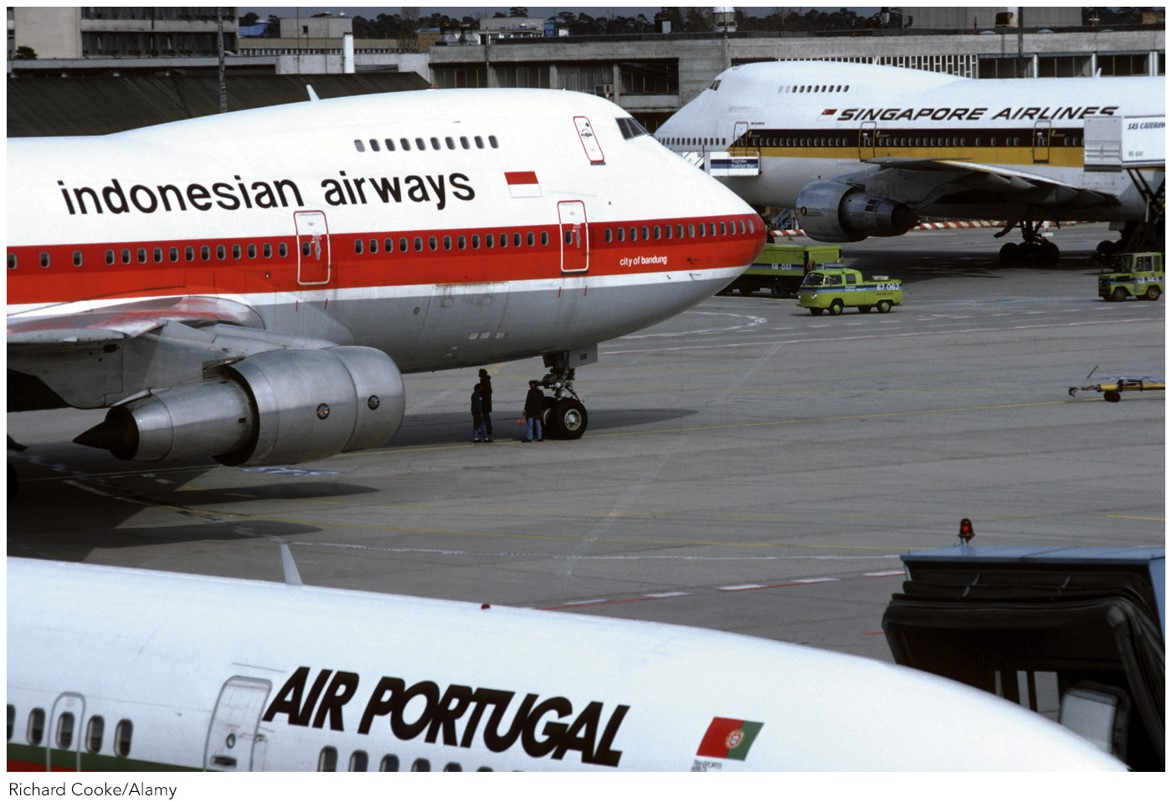
\includegraphics[width=\textwidth,height=\textheight,keepaspectratio]{ICAO.jpg}
\end{frame}

\begin{frame} 
	\frametitle{\LARGE{Types of Intl. Law}}
Two types of international law:
	\begin{enumerate}
		\item \textbf{Hard law}: precisely defined obligations with meaningful third-party delegation. Generally binding and enforceable. \pause
		\begin{itemize}
			\item Ex: Geneva Conventions, UNCLOS, GATT/WTO rules \pause
		\end{itemize}
	\end{enumerate}
States may act to enforce hard law via a variety of policy tools ranging from sanctions through military intervention.
\end{frame}

\begin{frame} 
	\frametitle{\LARGE{Types of Intl. Law}}
	Two types of international law:
	\begin{enumerate}
	  	\setcounter{enumi}{1}
		\item \textbf{Soft law}: lacks at least one characteristic of hard law; frequently imprecise with little meaningful delegation. \pause
		\begin{itemize}
			\item Ex: UN Framework Convention on Climate Change (prior to Kyoto Protocol) 
		\end{itemize}
	\end{enumerate}
	Soft law can become hard law over time as subsequent negotiations add more obligations. UNFCCC was soft law, but the Kyoto Protocol made it into hard law.
\end{frame}

\begin{frame} 
	\frametitle{\LARGE{Laws and Strategic Incentives}}
So, how and when do states create and follow international law? \pause
	\begin{itemize}
		\item \textbf{Selection effect concerns}: do states only create and follow those laws that align with what they were planning to do regardless? \pause
		\item States, especially powerful ones, have incentives to create favorable outcomes for themselves, \textit{including in interpretation and implementation of international law.} \pause
		\item The most powerful states may be able to act without the permission of international law (ex: 2003 Iraq War). \pause
		\item Despite this, international law is another institution that clarifies expectations and enables cooperation. 

	\end{itemize}
\end{frame}

\begin{frame} 
	\frametitle{\LARGE{Laws and Strategic Incentives}}
	So, how and when do states create and follow international law? 
	\begin{itemize}
		\item Empirically, compliance rates are high. \pause
		\item Laws can create opportunities for mutually beneficial cooperation. 
		\begin{itemize}
			\item Ex: In war, treating enemy POWs well creates an expectation that your enemy will treat your POWs well. \pause
		\end{itemize}
		\item Laws may also create \textbf{compliance constituencies}: groups within the state who benefit from that law, and so lobby the government to follow it. \pause
		\item \textbf{General consensus is that international law matters, but only if states perceive cooperative benefits from following it.}		
	\end{itemize}
\end{frame}


\begin{frame} 
	\frametitle{\LARGE{Norms Definition}}
	What about international norms? \pause
	\begin{itemize}
		\item \textbf{Norms}: behavior standards for a type of actor, dictating proper behavior in a given circumstance. \pause Subtypes:
		\begin{enumerate}
			\item Constitutive: defines a legitimate actors (ex: who counts as a state). \pause
			\item Procedural norms: similar to secondary rules; determine how multilateral decisions should be made. \pause
			\item Regulative norms: define acceptable behavior between actors. \pause
		\end{enumerate}
	\item Most discussions of norms are about regulative norms.
	\end{itemize}
\end{frame}

\begin{frame} 
	\frametitle{\LARGE{Norms vs. Laws}}
	\begin{itemize}
		\item \textbf{Norms are not laws.} \pause
		\item Norms may inspire international laws, but norms lack the formal aspects of international law. \pause
		\item Norms form as social constructions. \pause
		\item Additionally, some of the most important norms are so deeply embedded in society as to be invisible. \pause Ex: against cannibalism. \pause
		\item This means that studying norm formation and compliance is complicated.		
	\end{itemize}
\end{frame}

\begin{frame} 
	\frametitle{\LARGE{Norm Creation}}
	\begin{itemize}
		\item Norms, especially regulative norms, can arise over a long period of time in a similar way as customary law. \pause
		\begin{itemize}
			\item Ex: The ``nuclear taboo" against using nuclear weapons.
		\end{itemize}
		\item Norms can also arise in response to specific events (ex: Rwandan Genocide and R2P).
		\item Finally, norms can be deliberately built by \textbf{norms entrepreneurs}, who often lead and coordinate \textbf{transnational advocacy networks} campaigning for a specific norm (ex: end of child marriage or labor, abolition of slavery, etc.)
	\end{itemize}
\end{frame}

\begin{frame} 
	\frametitle{\LARGE{Norm Life Cycle}}
	\begin{itemize}
		\item \textbf{Convince} actors that the norm is important. This is more effective if the norm is linked to existing norms. \pause
		\begin{itemize}
			\item Often done by \textbf{transnational advocacy networks (TANs)}. \pause
		\end{itemize}
		\item \textbf{Cascade:}	At some point, norm becomes so widespread that it becomes generally accepted; this often speeds further adoption. AKA the ``tipping point.” \pause
		\item \textbf{Internalize:} Once norm is universally shared, often can become taken for granted and an unconscious influence on policymaking.		
	\end{itemize}
\end{frame}

\begin{frame} 
	\frametitle{\LARGE{Transnational Advocacy Networks}}
	\begin{itemize}
		\large{
			\item \textbf{Transnational advocacy networks} (TANs) are motivated by principles, and further these by being strategic actors. \pause
			\item Their goals are usually to change some form of government behavior or inaction. \pause 

			\item This is frequently achieved through monitoring states' compliance with international human rights commitments. \pause 

			\item TANs frequently engage in ``naming and shaming" using the boomerang model.
		}
	\end{itemize}
\end{frame}

\begin{frame} 
	\frametitle{\LARGE{Boomerang Model}}
	\begin{figure}[ht!]
		\centering
		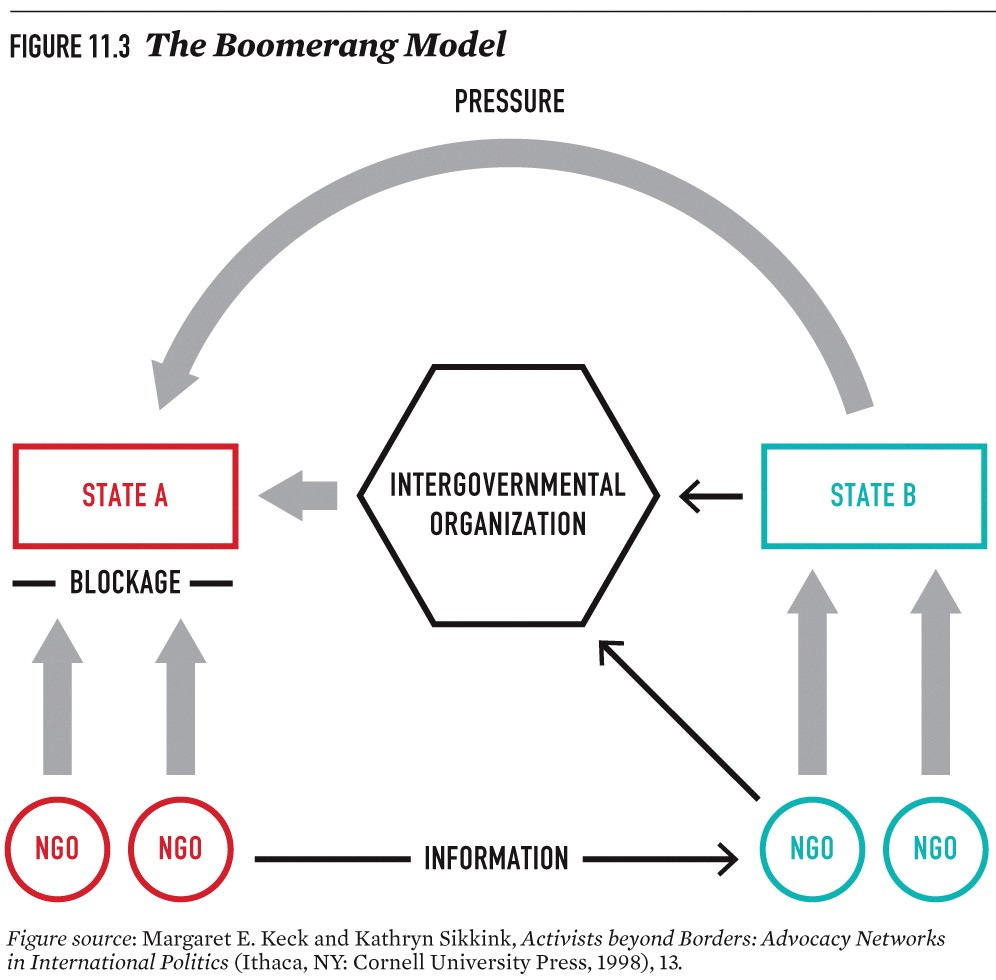
\includegraphics[width=\textwidth,height=0.9\textheight,keepaspectratio]{boomerang.jpg}
	\end{figure}
\end{frame}

\begin{frame} 
	\frametitle{\LARGE{Boomerang Model}}
	\begin{itemize}
		\item This model suggests that, when a domestic group does not expect a reaction from its own government, they can try to create outside pressure through triggering transnational action. \pause
		\item TANs frequently serve as \textbf{information shortcuts} here, quickly supplying information to foreign actors that can pressure the government.
		
	\end{itemize}
\end{frame}

\begin{frame} 
	\frametitle{\LARGE{Why Do Norms Matter?}}
	\begin{itemize}
		\item Norms have the potential to change the preferences and interests of states and other international actors. \pause
		\item Norms violations exposed by TANs (``naming and shaming") may impact a state's reputation and/or draw sanctions from other states, altering their interactions.
		\begin{itemize}
			\item Boomerang model is a primary example of this. \pause
		\end{itemize}
		\item Danger of unintended side effects. Ex: campaigns against child labor leading to children in unregulated illegal sweatshops.
		\item Norms have strongly influenced the development of human rights law.
	\end{itemize}
\end{frame}

\begin{frame} 
	\frametitle{\LARGE{Summary of Intl Law}}
	\begin{itemize}
		\item International law and norms are institutions.
		\item Law and norms can shape the interests of states.
		\item International law is most effective when it facilitates mutually beneficial cooperation.
		\item Norms can develop and change over time, and can motivate international laws.
		\item TANs promote normative values and pressure governments to follow them.	
	\end{itemize}
\end{frame}

\begin{frame} 
	\frametitle{\LARGE{Central Questions of Human Rights}}
	\centering
	\Large{What are human rights? Why do states undertake costly actions to protect human rights outside their borders?}
\end{frame}

\begin{frame} 
	\frametitle{\LARGE{What are Human Rights?}}
	\begin{itemize}
		\item \textbf{Human rights}: broadly speaking, those rights possessed by all individuals by virtue of their humanity. \pause
		
		\item Explicitly codified for the first time (ever!) with the 1948 Universal Declaration of Human Rights (UDHR). \pause
		\item UDHR motivated by horrors of WWII and the Holocaust.
		\item Since 1948, multilateral human rights treaties have proliferated.
		
	\end{itemize}
\end{frame}

\begin{frame}{\LARGE Human Rights Agreements}
	\centering
	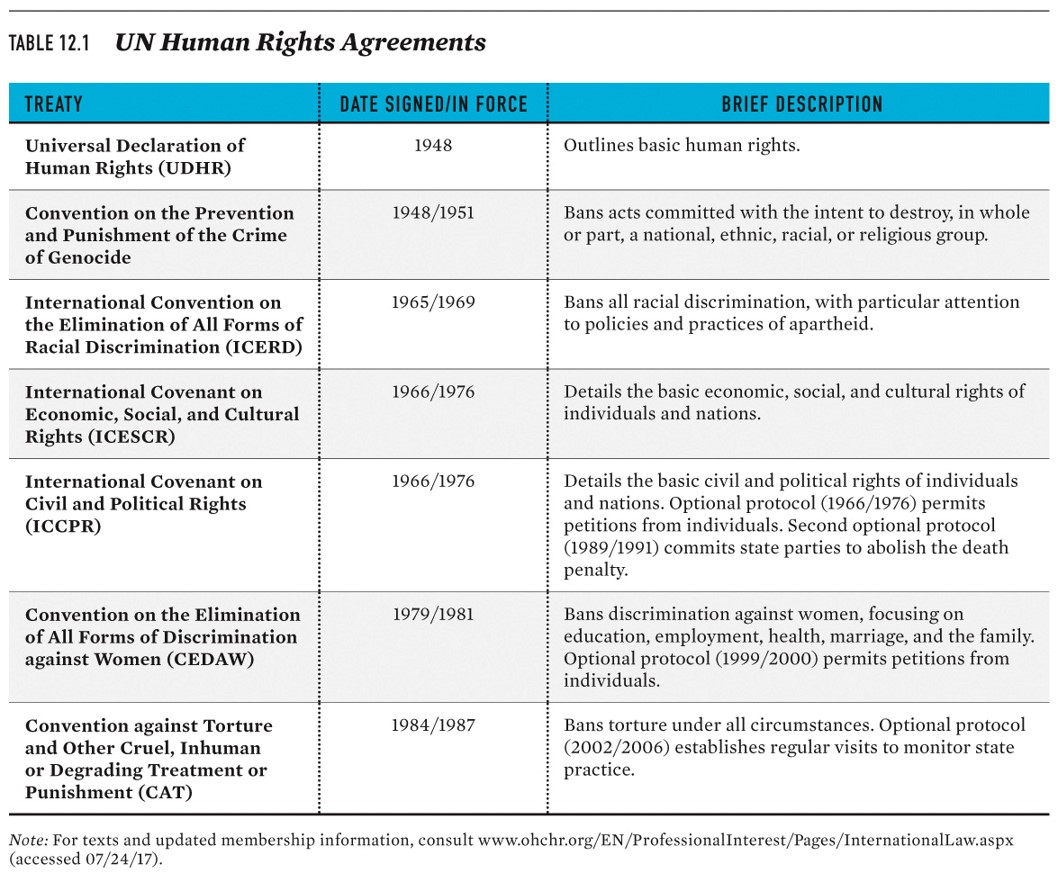
\includegraphics[width=\textwidth,height=0.9\textheight,keepaspectratio]{UNHR1.jpg}
\end{frame}

\begin{frame}{\LARGE Human Rights Agreements}
	\centering
	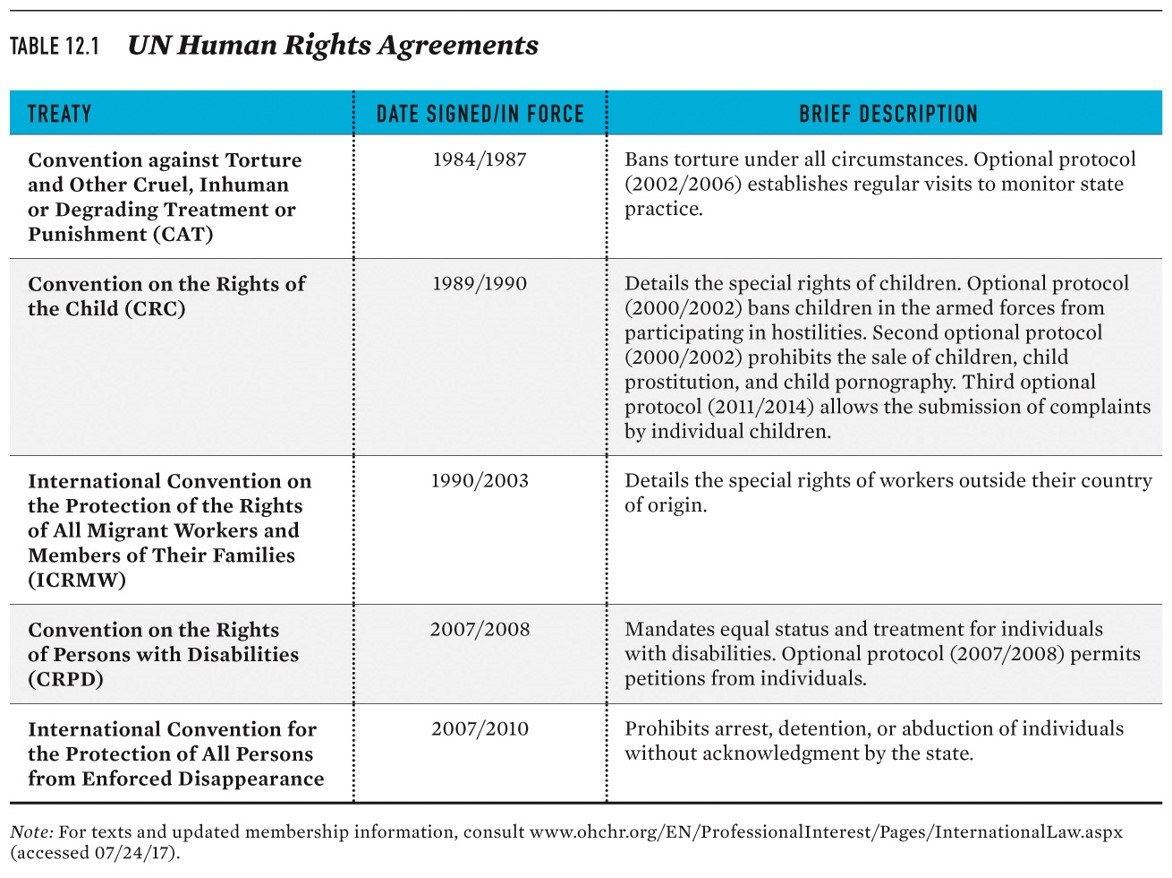
\includegraphics[width=\textwidth,height=0.9\textheight,keepaspectratio]{UNHR2.jpg}
\end{frame}

\begin{frame} 
	\frametitle{\LARGE{What Are Human Rights?}}
	\begin{itemize}
		\item Modern conceptions of human rights usually reflect Western ideals. \pause
		\item Heavily influenced by English philosopher John Locke's \textbf{natural rights}: by nature, humans are free and equal, possessing rights independent of those granted by the laws, customs, or beliefs of society or government. \pause
		\item Western ideals of human rights have tended to focus on the individual as the primary unit, emphasizing freedom and economic and social rights. \pause
		\begin{itemize}
			\item Note the tension with socialism's focus on the community during the Cold War, or the ``Asian values" discourse in the 1990s, which focused more heavily on collectivism and community. \pause
		\end{itemize}
		\item Modern human rights treaties tend to reflect Western ideals.		
	\end{itemize}
\end{frame}

\begin{frame} 
	\frametitle{\LARGE{What Are Human Rights?}}
	\begin{itemize}
		\item While human rights sound appealing in the abstract, defining the obligations of states with respect to human rights is much harder.
		\item Example: the right of every person to their life. \pause
		\item A basic understanding of this: you have no right to take away my life (and vice versa). \pause
		\item Most people would agree that this means murder is not to be tolerated. \pause
		\item But what about capital punishment (the death penalty)?	
	\end{itemize}
\end{frame}

\begin{frame} 
	\frametitle{\LARGE{Negative and Positive Rights}}
	Some philosophers also emphasize the difference between ``negative” and ``positive” rights. \pause
	\begin{itemize}
		\item \textbf{Negative right}: don't do things that limit the ability of others to enjoy a right. Generally prohibits certain actions.
		\begin{itemize}
			\item Ex: don't kill, don't torture, etc. \pause
		\end{itemize}
		\item \textbf{Positive right}: Defines actions that should be taken to ensure all individuals have equal opportunity to enjoy a right. \pause
		\begin{itemize}
			\item Ex: some activists have argued that, to fully enjoy the “right to life,” individuals also require material support. 
			\item It is difficult to live without a place to live of one’s own; thus, ``right to life” should include a right to have a home. 
		\end{itemize}
	\end{itemize}
\end{frame}

\begin{frame} 
	\frametitle{\LARGE{Postwar Human Rights Law Growth}}
	\begin{itemize}
		\item UDHR is aspirational soft law, but provides a set of standards for subsequent treaties. \pause
		\item UDHR was negotiated alongside the \textbf{Convention on the Prevention and Punishment of the Crime of Genocide (Genocide Convention)}, international hard law outlawing genocide. \pause
		\begin{itemize}
			\item Signed by US in 1948 but not ratified until 1988. Why? \pause Sovereignty concerns. \pause
		\end{itemize}
		\item Two legally binding agreements were born out of UDHR: the \textbf{ICCPR} and the \textbf{ICESCR}.
	\end{itemize}
\end{frame}

\begin{frame} 
	\frametitle{\LARGE{ICCPR and ICESCR}}
	\begin{itemize}
		\item \textbf{International Covenant on Civil and Political Rights (ICCPR)}: focus on civil and political rights (life, liberty, freedom of thought, religion, etc.) \pause
		\item \textbf{International Covenant on Economic, Social, and Cultural Rights (ICESCR)}: focuses on rights to minimum wages for dignified living, right to form unions, compensation for maternity leave, etc.	
		\item Combined with the UDHR, these two covenants form the \textbf{International Bill of Rights}.
	\end{itemize}
\end{frame}

\begin{frame} 
	\frametitle{\LARGE{Human Rights and America}}
	Consider America's relationship with these treaties...
	\begin{itemize}
		\item Signed the Genocide Convention in 1948 but did not ratify it until 1988 (\href{https://enoughproject.org/blog/day-us-ratifies-genocide-convention}{details}).
		\begin{itemize}
			\item The Convention is a non-self-executing treaty, meaning that it requires additional domestic legislation to actually turn its provisions into binding US law. \pause
		\end{itemize}
		\item US ratified the ICCPR in 1992 while also declaring it as non-self-executing, effectively not truly ratifying it at all.\pause
		\item US signed ICESCR in 1977 but never ratified it. 
	\end{itemize}
	
\end{frame}


%https://worldcoalition.org/campagne/just-one-more-step-ratifying-international-and-regional-protocols/
\begin{frame} 
	\frametitle{\LARGE{Human Rights and America}}
	\begin{itemize}
		\item The International Covenant on Civil and Political Rights’ (ICCPR) provisions for political and civil rights include limiting the death penalty to the most serious crimes. \pause
		\item ICCPR forbids death penalty entirely for those under 18 years old. \pause
		\item As of July 2023, 173 of the UN’s 193 member countries were parties to the ICCPR.
		\item 90 countries have signed an optional protocol of the ICCPR aimed at abolishing the death penalty, while 108 have completely abolished the death penalty (\href{https://www.aljazeera.com/news/2022/10/10/infographic-which-countries-still-have-the-death-penalty-2}{more info}). \pause
		\item The United States is an outlier among advanced industrialized states, and routinely condemned by Amnesty International for its use of capital punishment. 
	\end{itemize}
\end{frame}

%Protesters against US death penalty outside US embassy in Hong Kong
\begin{frame}{\LARGE Death Penalty Protests}
	\centering
	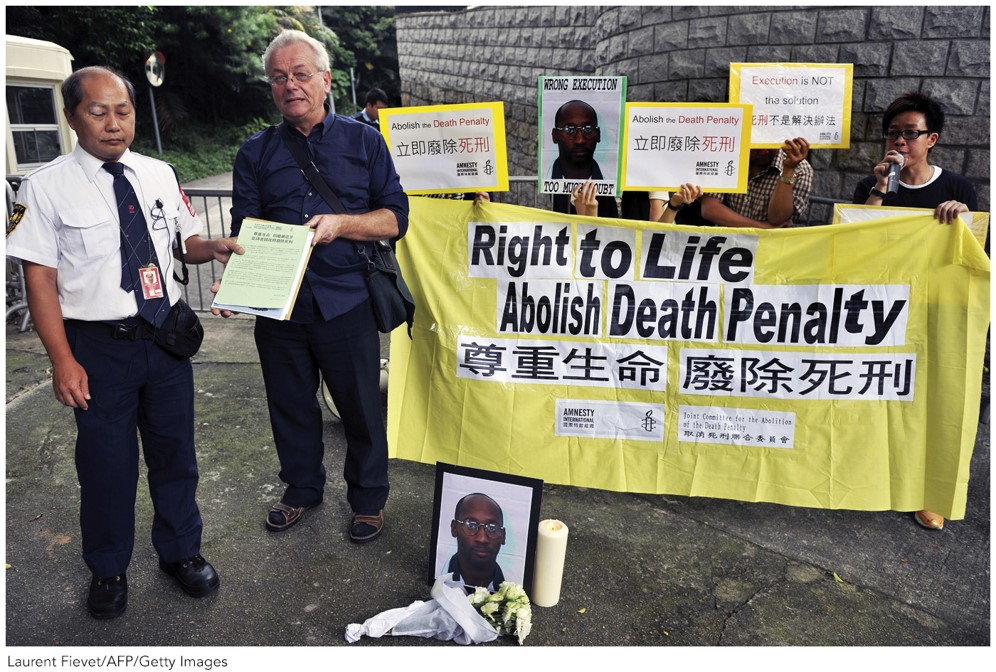
\includegraphics[width=\textwidth,height=0.9\textheight,keepaspectratio]{hongkongprotests.jpg}
\end{frame}


\begin{frame} 
	\frametitle{\LARGE{Why Are Human Rights Controversial?}}
	\begin{itemize}
		\item Why do states try to avoid fully following these treaties?
		\item \textbf{Fundamental tension between the idea of universal human rights and state sovereignty.} \pause
		\item The idea of human rights says that there are some actions states \textit{cannot take against their citizens}--that is, an external constraint on their sovereign authority. \pause
		\item Human rights can be weaponized politically at the international level (ex: Western vs. Communist emphasis on ICCPR vs. ICESCR during Cold War; civil rights viewed as Trojan Horse for Western influence).
	\end{itemize}
\end{frame}

\begin{frame} 
	\frametitle{\LARGE{Why Are Human Rights Controversial?}}
	\begin{itemize}
		\item Human rights provisions can also face domestic opposition from a variety of sources. \pause
		\begin{itemize}
			\item Policymakers may fear infringements on their state's sovereignty. \pause
			\item Certain human rights may be unpopular with voters (ex: \href{https://www.pewresearch.org/politics/2021/06/02/most-americans-favor-the-death-penalty-despite-concerns-about-its-administration/}{Pew polling} in 2021 and \href{https://news.gallup.com/poll/404975/steady-americans-support-death-penalty-murderers.aspx}{Gallup polling} in 2022 shows that a majority of Americans still favor the death penalty.) \pause
			\item Concerns about human rights as a means of spreading Western influence.
			
		\end{itemize}
	\end{itemize}
\end{frame}

\begin{frame} 
	\frametitle{\LARGE{Why Do States Violate Human Rights?}}
	\begin{itemize}
		\item Poor state capacity \pause
		
		\item National security (e.g. Red Scare, WWII Japanese internment camps, Guantanamo Bay) \pause
		
		\item Concerns over remaining in power (e.g. Dirty War in Argentina)\pause 
		
		\item Costs of violating treaties may be low due to lack of enforcement provisions \pause 
	\end{itemize}
	Autocracies and unstable democracies usually violate human rights more than consolidated democracies, but they are not immune...
\end{frame}

\begin{frame}{\LARGE Homelessness in America}
	\centering
	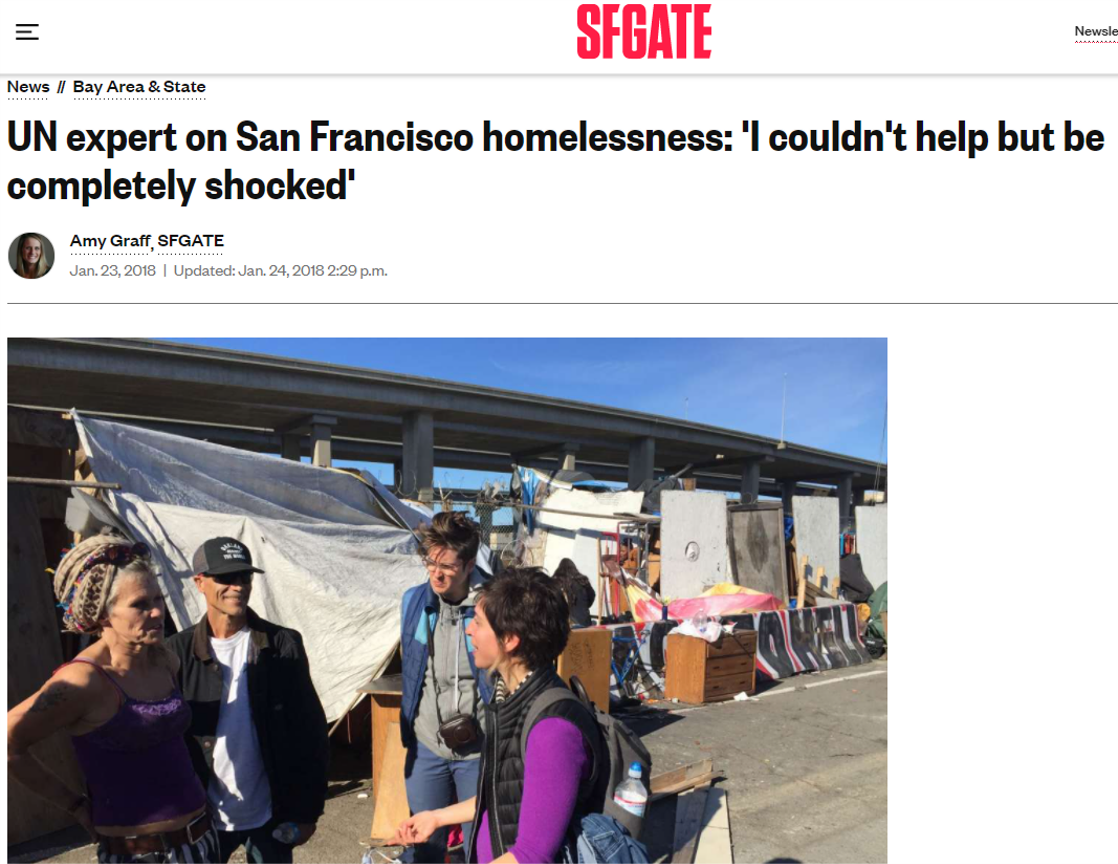
\includegraphics[width=\textwidth,height=0.9\textheight,keepaspectratio]{SFhomeless.png}
\end{frame}

\begin{frame}{\LARGE Homelessness in America}
	\begin{itemize}
		\item UN foreign observer visited San Francisco in 2018 as part of a global study on informal settlements (\href{https://www.sfgate.com/bayarea/article/Leilani-Farah-UN-rapporteur-homelessness-SF-CA-12519117.php}{article}). \pause
		\item Her assessment: ``If I could add, the other thing that just struck me ... but I'm sorry, California is a rich state, by any measures, the United States is a rich country, and to see these deplorable conditions that the government is allowing, by international human rights standards, it's unacceptable. I'm guided by human rights law.”
		
	\end{itemize}
\end{frame}


\begin{frame} 
	\frametitle{\LARGE{Why Sign Human Rights Agreements?}}
	States have a variety of reasons to sign these agreements:
	\begin{itemize}
		\item New democracies may want to institutionalize norms of human rights. \pause
		\item Issue linkage can also play a role: other states may offer aid, trade agreements, etc. conditional on a state joining. \pause 
		\item Signaling: states may sign treaties to signal to international investors that they are a safe/secure place to invest. Additionally, many regional trade agreements contain human rights clauses that have small but meaningful impacts. \pause
		\item States join agreements to try to constrain actions of other states via diplomatic pressure.
		
	\end{itemize}
\end{frame}

\begin{frame} 
	\frametitle{\LARGE{Why Care About Human Rights Abuses?}}
	Why would states be concerned about human rights abuses outside of their sovereign territory?
	\begin{itemize}
		\item Altruistic reasons: empathy for the disadvantaged, as framed by TAN advocacy and human rights advocates. \pause
		\item Strategic reasons: fear of conflict spillover, as civil wars and repression may lead to international refugee flows (ex: Syrian civil war). \pause 
		\item Domestic reasons: lobbying for improved human rights may directly or indirectly benefit domestic actors for altruistic or strategic reasons. \pause
		\begin{itemize}
			\item Ex: labor unions demanding human rights provisions in trade treaties, to prevent criminally exploited labor that is also cheaper than their own.
		\end{itemize} 
		
	\end{itemize}
\end{frame}




\begin{frame} 
	\frametitle{\LARGE{HR Enforcement}}
	\begin{itemize}
		\item Relatively few human rights violators are punished. \pause
		\item It is costly to punish violators, and enforcement may be a collective action problem; knowing this, states feel able to violate HR, especially if they are powerful. \pause
		\begin{itemize}
			\item Naming and shaming may provoke the target to retaliation. \pause
			\begin{itemize}
				\item Ex.:  Anti-NBA backlash in China over Hong Kong support (\href{https://www.businessinsider.com/nba-china-feud-timeline-daryl-morey-tweet-hong-kong-protests-2019-10}{info}).
				
			\end{itemize}
			\item Publicly denouncing HR violations may reduce a state's ability to cooperate on other areas of mutual interest. \pause
			\begin{itemize}
				\item US and China must cooperate on environmental protection measures.
			\end{itemize}
		\end{itemize}
	\end{itemize}
\end{frame}

\begin{frame} 
	\frametitle{\LARGE{HR Enforcement}}
	Under what conditions are states likely to enforce human rights?
	\begin{enumerate}
		\item Domestic demands for action, such as TAN lobbying. \pause
		\item If action against human rights abusers serves the country’s larger political interests. \pause
		\begin{itemize}
			\item Ex: US intervention in Iraq also helped strengthen petrodollar system. \pause
		\end{itemize}
		\item If action can be framed as consistent with the norms of sovereignty and noninterference. \pause 
		\begin{itemize}
			\item Ex: Anti-apartheid movement in South Africa was framed as anti-colonial struggle over domestic representation.
			\item Note: This is most likely to occur when there is significant request for help from local actors; not clear same case can be made without local groups asking for assistance.
			
		\end{itemize}
		
		
	\end{enumerate}
\end{frame}

\begin{frame} 
	\frametitle{\LARGE{Responsibility to Protect}}
	\begin{itemize}
		\item The question of enforcement was forced into the international community's attention by the Rwandan genocide in 1994. \pause
		\item The failure of the international community to effectively act, and attempts by major powers like the US to avoid acting, enabled the genocide to continue. \pause
		\item UN advocacy afterwards led to the 2001 articulation of \textbf{Responsibility to Protect (R2P)}: the international community is obligated to protect threatened populations from genocide, war crimes, ethnic cleansing. \pause
		\item R2P invoked to justify intervention in the Libyan civil war in 2011. \pause
		\item \textbf{Note the clash with the idea of state sovereignty.}
	\end{itemize}
\end{frame}

\begin{frame} 
	\frametitle{\LARGE{HR Violations and Punishment}}
	\begin{itemize}
		\item Economic sanctions are one of the most common forms of punishment in those cases where states do agree to punish violators. \pause
		\item Mixed findings in the literature on the effectiveness of sanctions (including smart sanctions targeting elites) and whether wide-ranging sanctions hurt the population. \pause
		\item Example:  after Iraq invaded Kuwait in Persian Gulf War in 1991, UNSC passed a resolution imposing sanctions on the Iraqi economy, banning exports to Iraq that were not basic food or medicine. \pause
		\item Sanctions did not force Saddam out of power, but had a serious impact on the wellbeing of average Iraqi citizens...		 
	\end{itemize}
\end{frame}

%Source: http://special.seattletimes.com/o/news/nation-world/usiraq/turmoil/sanctions.html

\begin{frame} 
	\frametitle{\LARGE{Sanction Consequences}}
	\begin{figure}[ht!]
		\centering
		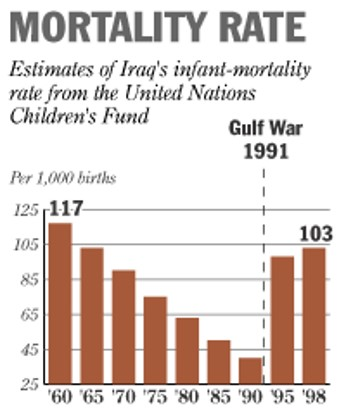
\includegraphics[width=\textwidth,height=0.8\textheight,keepaspectratio]{Iraqmortality.jpg}
	\end{figure}
\end{frame}

\begin{frame} 
	\frametitle{\LARGE{Do States Respect Human Rights?}}
	\begin{itemize}
		\item The legal framework for defining HR and punishing HR abuses is more developed than it has ever been in human history. \pause
		\item However, abuses still continue, even from states that have signed these treaties. \pause
		\item In addition to selection problem effects, the actual measurement of human rights is a murky subject. HR are frequently monitored and measured by TANs, as governments rarely advertise their abuses. \pause
		\item Developing HR standards over time further complicate measurement. \pause
		\item Determining effectiveness of agreements is a complex task. \pause
		\item Despite all this, human rights respect is (probably) improving over time. One reason for hope is the ICC...
		
		
	\end{itemize}
\end{frame}



\begin{frame} 
	\frametitle{\LARGE{Measuring Human Rights}}
	\begin{figure}[ht!]
		\centering
		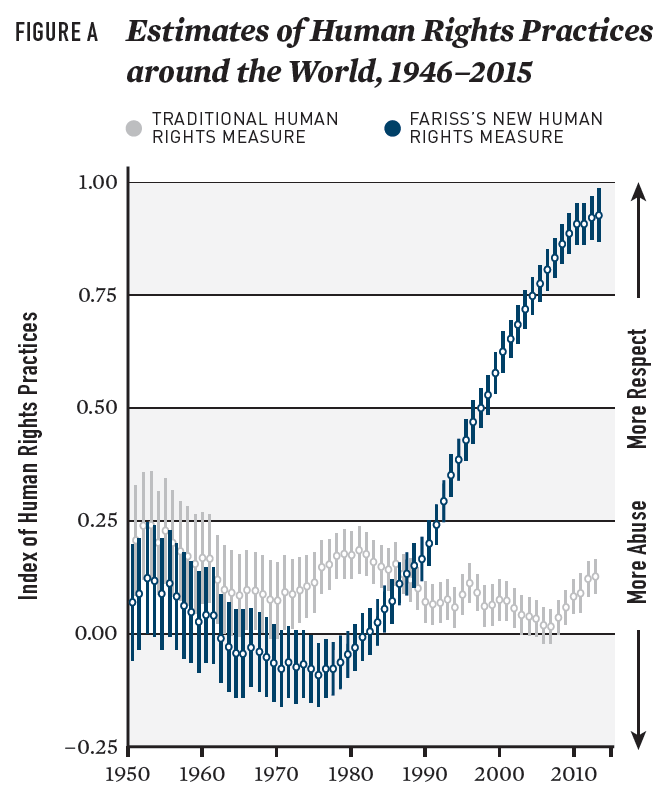
\includegraphics[width=\textwidth,height=0.9\textheight,keepaspectratio]{./farriss.png}
	\end{figure}
\end{frame}


\begin{frame} 
	\frametitle{\LARGE{The International Criminal Court}}
	\begin{itemize}
		\item Some states grant in their constitutions the right of individual citizens to appeal to international bodies for final jurisdiction in rights cases (but remember selection effects). 
		\item They usually appeal to the \textbf{International Criminal Court}.
		\begin{itemize}
			\item The ICC can try individuals for war crimes and threats to peace.
			\item Before the ICC’s creation in 1998, only states could be tried.
			\item Though more than 100 states have accepted the jurisdiction of the ICC since it was established in 1998, the United States refuses to join. 
			\item As of November 2023, 31 cases have been brought before the court for investigation and trial.
		\end{itemize}
	\end{itemize}
\end{frame}

\begin{frame} 
	\frametitle{\LARGE{The International Criminal Court}}
	\begin{itemize}
		\item ICC's first conviction was in March 2012 of Thomas Lubanga Dylio, sentenced to 14 years for forcibly recruiting child soldiers in the DRC. \pause
		\item Ratification of the ICC and prosecutions by the Court have been found to reduce state sponsored violence, while prosecutions reduce rebel group abuses. \pause
		\item Other research has found that that involvement of the ICC in a conflict prolongs the strife and killings, especially when the risk of domestic prosecution is relatively low.
		\begin{itemize}
			\item Risk of prosecution may motivate factional leaders to fight on longer than they would otherwise.
		\end{itemize}
		\item ICC also criticized for its focus on Africa.	
	\end{itemize}
\end{frame}

\begin{frame} 
	\frametitle{\LARGE{Summary of Human Rights}}
	\begin{itemize}
		\item Most of the international system agrees in principle on what most human rights are, most of the time. \pause
		\item States are most likely to respect the human rights of their citizens when those rights are strongly institutionalized and violation would lead to negative economic and political consequences (sanctions, denunciations, loss of cooperation, etc.). \pause
		\item States are most likely to act to enforce human rights outside of their own territory if domestic actors/TANs effectively lobby for it, enforcement serves strategic goals, and enforcement does not violate sovereignty norms. \pause
		\item Respect for human rights may be increasing over time; institutions such as the ICC probably help.
	\end{itemize}
\end{frame}


\end{document}